\documentclass[12pt]{article}

\RequirePackage{amsmath}
\RequirePackage{amsthm}
\RequirePackage{amssymb}
\RequirePackage[mathscr]{eucal}
\RequirePackage{mathtools}
\RequirePackage{etoolbox}

\usepackage[blue]{zhoucx-notation}

\usetikzlibrary{arrows.meta,angles,quotes}
\colorlet{linecol}{black!75}
\usepackage{forest}

\geometry{letterpaper, top = 1in, bottom = 1in, left = 1.5in, right = 1in}

% correct bad hyphenation here
\hyphenation{op-tical net-works semi-conduc-tor}
\theoremstyle{definition}
\newtheorem{definition}{Definition}
%\declaretheorem[numbered=no]{definition}

\theoremstyle{theorem}
\newtheorem{lemma}{Lemma}
\newtheorem{proposition}{Proposition}
\newtheorem{conjecture}{Conjecture}
\newtheorem{theorem}{Theorem}
\newtheorem{corollary}{Corollary}

\theoremstyle{remark}
\newtheorem{remark}{Remark}
\newtheorem{example}{Example}

\renewcommand{\qedsymbol}{\hfill\rule{2mm}{2mm}}

%\pagestyle{fancy}
%\fancyhf{}
%\setlength{\headheight}{15pt}
%\rhead{\textsf{June 12, 2022}}
%\lhead{\textsf{Chenxi Zhou}}
%\renewcommand{\headrulewidth}{1pt}
\cfoot{\thepage}

\setstretch{2}

\title{\Large \textbf{Chapter 1: Introduction}}
\author{}
\date{}

\begin{document}

\thispagestyle{plain}
\maketitle

\tableofcontents

% --------------------------------------------------------------------

\newpage

Density estimation is a classical and fundamental problem in statistics. With independent and identically distributed (iid) data drawn from an unknown probability density function (pdf) $p_0$ over a domain $\calX \subseteq \Real^d$, the \emph{density estimation problem} seeks to reconstruct $p_0$ from these observations \parencite{Silverman1986-mu}. 

Density estimation has found a wide range of applications. On one hand, density estimates can be used in exploratory data analysis. More specifically, they can be utilized as an informal investigation of the properties of a given dataset and provide descriptive features such as multimodality, skewness, and tail behavior \parencite{Silverman1986-mu, Izenman2009-jk}. On the other hand, density estimates can be used as an intermediate step to perform further statistical analysis, such as classification \parencites{Ripley1996-bi} and clustering \parencites{Fukunaga1975-vy}. Due to its wide applications, there have been a plenty of works contributing to this problem. 

We will provide a review of different approaches to the density estimation problem and discuss their advantages and disadvantages in Section \ref{section-methods}. We then turn to the focus of this dissertation, density estimation in an exponential family induced by a reproducing kernel Hilbert space (RKHS), and introduce the problems we consider in this dissertation in Section \ref{section-our-focus}. The organization of the rest of this dissertation will be given in Section \ref{section-organization}. 

\section{An Review of Density Estimation Methods}\label{section-methods}

Existing density estimation methods can be broadly categorized into the parametric approach (Subsection \ref{subsection-parametric-density-estimation}) and the nonparametric approach (Subsection \ref{section-nonparam-approach}). The parametric approach imposes a strong assumption that $p_0$ belongs to a parametric family known up to a few parameters, %takes on a certain mathematical form of the hypothetical population from which the random sample is to be regarded as drawn. 
whereas the nonparametric approach abandons such a restrictive constraint and makes much fewer assumptions about $p_0$, which allows data to speak for themselves and offers more flexibility. 

In the remaining part of this section, we provide details of these two different approaches and discuss their advantages and disadvantages. 

\subsection{Parametric Approach}\label{subsection-parametric-density-estimation}

For the parametric approach, we assume $p_0$ belongs to a parametric family 
\begin{align}\label{eq-para-model}
	\calQ_{\mathrm{para}} := \sets[\Big]{p \parens{\,\cdot\,; \theta}: \calX \to [0, \infty) \bigm| \theta \in \Theta}, 
\end{align}
where $\theta := \parens{\theta_1, \cdots, \theta_m}^\top$ is an $m$-dimensional parameter and $\Theta \subseteq \Real^m$ is the parameter space; that is, we assume there exists $\theta^* \in \Theta$ such that $p_0 = p \parens{\,\cdot\,; \theta^*}$. The density estimation problem then reduces to a parameter estimation problem. Once we obtain an estimator of the parameter, say $\hat{\theta}$, the resulting density estimator is $p \parens{\,\cdot\,; \hat{\theta}}$. 

Many methods for estimating $\theta$ are available, for example, the method of moments and the method of maximum likelihood. 
%More precisely, with i.i.d samples $X_1, \cdots, X_n$ from $p^*$, the method of moments estimators equates the first $m$ sample moments to the corresponding population moments and solves the resulting system of $m$ equations 
%\begin{align*}
%	\E \parens{X^j} = \int_{\calX} x^j p \parens{x; \hat{\btheta}_{\mathrm{MOM}}} \diff x \stackrel{\text{set}}{=} \frac{1}{n} \sum_{i=1}^n X_i^j \hspace{20pt} \text{ for } j = 1, \cdots, m, 
%\end{align*}
The latter method, first proposed by \textcites{Fisher1922-qi}, considers to maximize the likelihood function
\begin{align}\label{eq-para-mle}
	\prod_{i=1}^n p \parens{X_i; \theta}, \qquad \text{ subject to } \theta \in \Theta, 
\end{align}
or, equivalently, maximize the (averaged) log-likelihood function
\begin{align}\label{eq-para-mle-log}
	\frac{1}{n} \sum_{i=1}^n \log p \parens{X_i; \theta}, \qquad \text{ subject to } \theta \in \Theta. 
\end{align}
The maximum likelihood estimator, denoted by $\hat{\theta}_{\MLE}$, is any point in $\Theta$ maximizing \eqref{eq-para-mle} or \eqref{eq-para-mle-log}. 

Since the functional form of density functions in $\calQ_{\mathrm{para}}$ is known, $\hat{\theta}_{\MLE}$ is generally very easy to compute, which either has an analytic form (e.g., when $\calQ_{\mathrm{para}}$ is the family of Gaussian pdfs with unknown mean and covariance matrix) or amounts to solving an optimization problem of dimensionality at most $m$. 

Statistical properties of these estimators have been well understood. For example, under certain regularity conditions, $\hat{\theta}_{\MLE}$ can be shown to be consistent, asymptotically efficient, and asymptotically normally distributed \parencite{Casella2002-vu}. 
% , Keener2010-en, Bickel2015-et}. 
%and details can be found, for instance, in Chapters 7 and 10 in \cite{Casella2002-vu}, Chapters 8 and 9 in \cite{Keener2010-en}, and Chapters 2, 5 and 6 in \cite{Bickel2015-et}. 
Some of these favorable statistical properties can be extended to density estimators under additional assumptions. 
%Supposing, for example, density functions in $\calQ_{\mathrm{para}}$ satisfy the Lipschitz condition  
%\begin{align*}
%	\norm[\big]{p \parens{\,\cdot\,; \theta_1} - p \parens{\,\cdot\,; \theta_2}} \le M \norm[\big]{\theta_1 - \theta_2}_2, \qquad \text{ for all } \theta_1, \theta_2 \in \Theta, 
%\end{align*}
%where $\norm{\,\cdot\,}$ is a norm measuring the distance between density functions in $\calQ_{\mathrm{para}}$, $\norm{\,\cdot\,}_2$ is the usual Euclidean distance, and $M > 0$ is a constant, we can show $p \parens{\,\cdot\,; \hat{\theta}_{\MLE}}$ converges to $p^* = p \parens{\,\cdot\,; \theta^*}$ under the norm $\norm{\,\cdot\,}$, since 
%\begin{align*}
%	0 \le \norm[\big]{p \parens{\,\cdot\,; \hat{\theta}_{\MLE}} - p \parens{\,\cdot\,; \theta^*}} \le M \norm[\big]{\hat{\theta}_{\MLE} - \theta^*}_2 \to 0, \qquad \text{ as } n \to \infty. 
%\end{align*}

Although density estimators from this parametric approach have computational advantages and possess many nice statistical properties, this approach relies on the rigid assumption $p_0 \in \calQ_{\mathrm{para}}$, which is hard or even impossible to verify in practice and is ``entirely a matter for the practical statistician'' \parencite{Fisher1922-qi}. If $p_0 \notin \calQ_{\mathrm{para}}$, the resulting density estimator from $\calQ_{\mathrm{para}}$ can be misleading and can lead to serious misspecification issues, which has been discussed by \textcites{Huber1967-sd, White1982-dn}. Therefore, \textcite{Fisher1922-qi} suggested to perform \textit{a posteriori} test to examine the adequacy of the parametric assumption and the potential existence of misspecification. 

\subsection{Nonparametric Approach}\label{section-nonparam-approach}

If a parametric model is not postulated, we pursue the nonparametric approach and make as few assumptions as possible about $p_0$. This is the focus of this dissertation. In particular, we focus on nonparametric methods via minimizing a loss functional plus a penalty functional over a class of pdfs, 
\begin{align}\label{eq-nonpara-general-problem} 
		\minimize_{q \in \calQ} \braces[\bigg]{ \widehat{L} \parens{q} + \lambda P \parens{q} }, 
\end{align}
where $\calQ$ is a pre-specified class of pdfs over $\calX$, $\widehat{L}: \calQ \to \Real$ is a loss functional, $P: \calQ \to [0, \infty)$ is a penalty functional, and $\lambda > 0$ is the penalty parameter. In \eqref{eq-nonpara-general-problem}, $\widehat{L}$ depends on data and measures the goodness-of-fit of $q$ to data, and the smaller $\widehat{L} \parens{q}$ is, the better the fit of $q$ to data is; and $P$ is typically independent of data and measures the smoothness or size of $q$, and the larger $P \parens{q}$ is, the less smooth or the more complex $q$ is. Hence, the objective functional in \eqref{eq-nonpara-general-problem} represents two conflicting goals: we demand $q$ to have a good fit to data, but we also require it to contain less variations and be not too complex. The penalty parameter $\lambda$ controls the tradeoff between these two conflicting goals. 

We will focus on two different choices of $\widehat{L}$, namely the negative log-likelihood loss functional (Subsection \ref{subsection-nonpara-mle}) and the score matching loss functional (Subsection \ref{subsection-nonpara-scorematching}). 

\subsubsection{Nonparametric Maximum Likelihood Density Estimation}\label{subsection-nonpara-mle}

Throughout this subsection, we let $\widehat{L}$ in \eqref{eq-nonpara-general-problem} be the (averaged) negative log-likelihood (NLL) loss functional 
\begin{align}\label{eq-nll-loss-function}
	\widehat{L}_{\NLL} \parens{q} := - \frac{1}{n} \sum_{i=1}^n \log q \parens{X_i}. 
\end{align}
We call the density estimator via minimizing $\widehat{L}_{\NLL}$ the maximum likelihood (ML) density estimator, as minimizing the NLL loss functional is equivalent to maximizing the log-likelihood functional. 

Minimizing $\widehat{L}_{\NLL}$ can be viewed as minimizing a sample version of the \textit{Kullback-Leibler divergence} (KL-divergence) 
\begin{align}
	\KLdiv \parens{p \Vert q} := \int_{\calX} p \parens{x} \log \parens[\bigg]{\frac{p \parens{x}}{q \parens{x}}} \diff x, 
\end{align}
where $p$ and $q$ are two probability density functions over $\calX$ and satisfy $\KLdiv \parens{p \Vert q} < \infty$. To see this, assuming $\KLdiv \parens{p_0 \Vert q} < \infty$ for all $q \in \calQ$, with a large $n$ and $X_1, \cdots, X_n \iid p_0$, we can approximate $\KLdiv \parens{p_0 \Vert q}$ by 
\begin{align*}
	\frac{1}{n} \sum_{i=1}^n \parens[\big]{\log p_0 \parens{X_i} - \log q \parens{X_i}} = & \, \frac{1}{n} \sum_{i=1}^n \log p_0 \parens{X_i} - \frac{1}{n} \sum_{i=1}^n \log q \parens{X_i} \\ 
	= & \,  \frac{1}{n} \sum_{i=1}^n \log p_0 \parens{X_i} + \widehat{L}_{\NLL} \parens{q}. 
\end{align*}
Notice that $\frac{1}{n} \sum_{i=1}^n \log p_0 \parens{X_i}$ is independent of $q$. The desired conclusion follows. 

If we let $\calQ$ be the class of all pdfs over $\calX$ and $P \parens{q} = 0$ for all $q \in \calQ$, $\widehat{L}_{\NLL}$ is unbounded below. To see this, suppose $\calX = \Real$ and let 
\begin{align*}
	q_{\sigma^2} \parens{x} = \frac{1}{n} \sum_{j=1}^n \frac{1}{\sqrt{2 \pi \sigma^2}} \exp \parens[\bigg]{-\frac{1}{2\sigma^2} \parens{x - X_j}^2}, \qquad \text{ for all } x \in \Real, 
\end{align*}
where $\sigma^2 > 0$. It is easy to verify that $q_{\sigma^2}$ is a valid pdf over $\Real$. Then, by shrinking $\sigma^2 \to 0$, we have $\widehat{L}_{\NLL} \parens{q_{\sigma^2}} \to - \infty$. 

Therefore, in order to obtain a sensible density estimator using $\widehat{L}_{\NLL}$, we need to impose certain constraints on $\calQ$ and/or choose a nonzero $P$. Several proposals have been made in the literature. 
%
%\subsubsubsection{Histogram density estimator}
%
%Suppose $\calX = \bracks{a, b}$, where $- \infty < a < b < \infty$, and let $\calQ$ be 
%\begin{align}\label{eq-class-histogram}
%	\sets[\Bigg]{q \biggm| q \parens{x} := \sum_{j=1}^m y_j \indic_{B_j} \parens{x}, y_j \ge 0 \text{ for all } j = 1, \cdots, m, \sum_{j=1}^m y_j = \frac{m}{b - a}}, 
%\end{align}
%where $m$ is a fixed positive integer, $\indic_A \parens{\,\cdot\,}$ is the indicator function of the set $A$, and 
%\begin{align*}
%	B_1 = \bigg[a, \frac{b-a}{m} \bigg), \hspace{5pt} B_2 = \bigg[\frac{b-a}{m}, \frac{2 \parens{b-a}}{m} \bigg), \hspace{5pt} \cdots, \hspace{5pt} B_m = \bigg[\frac{\parens{m-1} \parens{b-a}}{m}, b - a \bigg]. 
%\end{align*}
%%In addition, we let $P \parens{q} \equiv 0$. 
%Then, the maximizer of $\widehat{L}_{\NLL}$ over \eqref{eq-class-histogram} is the histogram density estimator. 
%
%The choice of the number of bins $m$, or equivalently, the choice of the bin width $\frac{b-a}{m}$, is critical in producing a good histogram, which is essentially a bias-variance trade-off problem. Too many bins, corresponding to too small bin width, lead to a histogram with low bias and high variance and result in undersmoothing; nonetheless, too few bins, corresponding to too large bin width, lead to a histogram with high bias and low variance and result in oversmoothing. Theoretically, the optimal bin width is $C \parens{p_0} n^{-\frac{1}{3}}$, leading to the asymptotic mean integrated squared error between the histogram density estimator and $p_0$ to be $\calO \parens{n^{-\frac{2}{3}}}$, where $C \parens{p_0}$ is a positive constant depending on $p_0$ \parencite{Wasserman2006-lj}. 
%
%Since the optimal bin width above depends on $p_0$, which is indeed the quantity of interest, it is only of theoretical interest and cannot be used in practice. There have been many alternative rules proposed. Motivated by minimizing the expected squared $L^2$ distance between the histogram density estimator and $p_0$, \textcite{Freedman1981-oi} proposed to choose the bin width to be $2 n^{-\frac{1}{3}} \mathrm{IQR} \parens{X_1, \cdots, X_n}$ that depends on the data only, where $\mathrm{IQR} \parens{X_1, \cdots, X_n}$ denotes the interquartile range of the data. 
%
%The histogram density estimator can be used as a convenient tool for data visualization in applications, but it does have several drawbacks. First, the histogram is constructed based on the assumption that the density value is identical in each bin, which is rather restrictive and sometimes even unrealistic. Second, the histogram density estimator is not smooth and has jumps at the boundaries of two adjoining bins. Therefore, alternative density estimators are needed. 

\subsubsubsection{Penalized Maximum Likelihood Density Estimation}

In their seminal paper, \textcite{Good1971-gm} proposed to use a nonzero $P$ and solve 
\begin{equation}\label{eq-good-gaskins}
	\begin{aligned}
		\minimize_{\gamma} & \, - \frac{1}{n} \sum_{i=1}^n \log \gamma^2 \parens{X_i} +  \parens[\bigg]{\lambda_1 \int_{\calX} \parens{\gamma' \parens{x}}^2 \diff x + \lambda_2 \int_{\calX} \parens{\gamma'' \parens{x}}^2 \diff x  }, \\ 
		\text{ subject to } & \, \int_{\calX} \gamma^2 \parens{x} \diff x = 1, 
	\end{aligned}
\end{equation}
where $\gamma^2 = q$, $\lambda_1 > 0$, and $\lambda_2 > 0$. The specific form of the penalty functional in \eqref{eq-good-gaskins} is motivated from penalizing both the slope and the curvature so that the resulting density estimates are very smooth. 

There are at least two advantages of working with $\gamma$ rather than the pdf $q$. Note that functions $\gamma$ and $q$ are related by $q = \gamma^2$. Thus, if $\hat{\gamma}$ is a solution to \eqref{eq-good-gaskins}, the resulting density estimator is $\hat{\gamma}^2$, which is automatically nonnegative over $\calX$. 

Furthermore, due to the constraint $\int_{\calX} \gamma^2 \parens{x} \diff x = 1$, $\gamma$ must belong to $L^2 \parens{\calX}$, the class of square-integrable functions over $\calX$, which is a Hilbert space. This provides computational convenience that one can exploit to compute the minimizer of \eqref{eq-good-gaskins}. Supposing $\sets{\varphi_j}_{j \in \Natural}$ is an orthonormal basis of $L^2 \parens{\calX}$, we can then approximate any $\gamma \in L^2 \parens{\calX}$ by $\gamma \approx \sum_{j=1}^{m} c_j \varphi_j$, for a large $m$. As a result, the minimization problem \eqref{eq-good-gaskins} over $L^2 \parens{\calX}$, an infinite-dimensional class of functions, reduces to a computationally tractable problem over $\Real^m$, as one only needs to determine the values of $c_1, \cdots, c_m$. The value of $m$ can be determined via cross validation or through an iterative fashion as \textcites{Good1971-gm} did. 

When solving \eqref{eq-good-gaskins}, one has to deal with the constraint $\int_{\calX} \gamma^2 \parens{x} \diff x = 1$, which can be difficult in practice. In order to remedy this, \textcites{Leonard1978-mc} introduced the logistic transformation of the density function, proposed to parametrize $q$ as $q = \exp \parens{f} / \int_{\calX} \exp \parens{f \parens{t}} \diff t$, and considered to minimize 
\begin{align}\label{eq-leonard}
	- \frac{1}{n} \sum_{i=1}^n f \parens{X_i} + \log \parens[\bigg]{\int_{\calX} \exp\parens{f \parens{x}} \diff x} + \frac{\lambda}{2} \widetilde{P} \parens{f}, \qquad \text{ subject to } f \in \calH, 
\end{align}
where $\calH$ is a pre-specified class of functions mapping from $\calX$ to $\Real$ and $\widetilde{P} \parens{f} = P \parens{q}$. If the solution to \eqref{eq-leonard} is $\hat{f}$, the resulting density estimator is $\exp \parens{\hat{f} \parens{x}} / \int_{\calX} \exp \parens{\hat{f} \parens{t}} \diff t$, for all $x \in \calX$, which is nonnegative over $\calX$ and integrates to 1. 

The main disadvantage of the formulation \eqref{eq-leonard} is that it may \textit{not} have a unique solution, since, if $\hat{f}$ is a solution, then $\hat{f} + c$ is a solution as well, for any $c \in \Real$. To remedy this, \textcite{Silverman1982-ey} proposed to minimize 
\begin{align}\label{eq-silverman}
	- \frac{1}{n} \sum_{i=1}^n f \parens{X_i} + \int_{\calX} \exp \parens{f \parens{x}} \diff x + \frac{\lambda}{2} \widetilde{P} \parens{f}, \qquad \text{ subject to } f \in \calH, 
\end{align}
which has a unique minimizer. Assuming $\widetilde{P}$ depends only on the square of derivatives of $f$, \textcite{Silverman1982-ey} proved the minimizer of \eqref{eq-silverman} exists, and showed, if $\hat{f}$ is the solution to \eqref{eq-silverman}, $\exp \parens{\hat{f}}$ is automatically the density estimator. Moreover, \textcite{Silverman1982-ey} established the consistency and the asymptotic convergence rate of his estimator under various function norms. However, no practical algorithms were proposed to compute his density estimator. 

Penalty functionals appearing in \eqref{eq-good-gaskins} and \eqref{eq-silverman} depend on the squared $L^2$ norm of the derivatives of the root-density or a transformation of the log-density. This is computationally convenient as the corresponding objective functional is differentiable so that first- and second-order iterative optimization algorithms can be applied to compute the respective minimizers and the resulting density estimators. Such penalty functionals, nonetheless, allow no jumps or piecewise linear bends in density estimates and often lead to over-smoothed density estimates \parencites{Sardy2010-hp}. Motivated by these observations, \textcites{Koenker2007-zo} considered the problem \eqref{eq-silverman} and chose $\widetilde{P}$ to be the total variation of $f'$, 
\begin{align}\label{eq-tv-koenker}
	\widetilde{P} \parens{f} = \sup \sum_{i=1}^m \abs{f' \parens{u_i} - f' \parens{u_{i-1}}}, 
\end{align}
where the supremum is taken over all partitions of $u_1 < u_2 < \cdots < u_m$ in $\calX \subset \Real$. 
%Note that the $\Phi$ \eqref{eq-tv-koenker} implies the resulting density estimate is at least differentiable. 
% Due to the choice of \eqref{eq-tv-koenker}, the resulting optimization problem is \emph{not} differentiable, and iterative optimization algorithms relying on derivatives cannot be applied. 
To facilitate the computation, \textcite{Koenker2007-zo} assumed $f$ is a piecewise linear function supported on $\bracks{X_{\parens{1}}, X_{\parens{n}}}$ with knots at the order statistics $X_{\parens{1}}, \cdots, X_{\parens{n}}$ and proposed to use the interior point method to compute the minimizer. 
%\textcite{Sardy2010-hp} considered the same problem and chose $\widetilde{P}$ to be the total variation of $f$ itself, and proposed a dual block coordinate relaxation method to compute the minimizer. 
From their simulation studies, \textcite{Koenker2007-zo} found that density estimates using the penalty functional \eqref{eq-tv-koenker} are capable of capturing sharp peaks in $p_0$ and work particularly well when $p_0$ is not smooth. However, theoretical properties of their density estimator, such as consistency and the rate of convergence, remain unexplored. 

\subsubsubsection{Shape-Constrained Maximum Likelihood Density Estimation}

Even though density estimators by minimizing $\widehat{L}_{\NLL}$ plus a penalty functional have very nice statistical properties, the quality of density estimates depends heavily on the choice of the penalty parameter $\lambda > 0$, which is a nontrivial task in general. 

A different direction of estimating $p_0$ via minimizing $\widehat{L}_{\NLL}$ is to impose certain qualitative properties on $p_0$, such as monotonicity, unimodality, or log-concavity. This shape-constrained approach is attractive as it requires no choice of penalty parameter and is fully automatic \parencite{Cule2010-lc}. 

Shape-constrained density estimation originated from \textcite{Grenander1956-db}, who studied the problem of estimating a non-increasing pdf over $[0, \infty)$ via minimizing $L_{\NLL}$. It turns out that the solution, called the \textit{Grenander estimator}, exists and is the left derivative of the \textit{least concave majorant} of the empirical distribution function $\widehat{F}_n$, 
%that is, 
%\begin{align}
%	\hat{p}_{\mathrm{Grenander}} \parens{x} := & \, \begin{cases}
%		\sup_{v > x} \inf_{u < x} \dfrac{\hat{F}_n \parens{v} - \hat{F}_n \parens{u}}{v - u}, & \, \text{ for } X_{\parens{0}} < x < X_{\parens{n}}, \\ 
%		0, & \, \text{otherwise}, 
%	\end{cases} \\ 
%	= & \, \begin{cases}
%		\hat{p}_{\mathrm{Grenander}} \parens{X_{\parens{i+1}}}, & \, \text{ for } X_i < x \le X_{i+1}, 0 \le i \le n-1, \\ 
%		0, & \, \text{ otherwise}, 
%	\end{cases}
%\end{align}
%where $X_{\parens{0}} = 0$, $X_{\parens{1}} < X_{\parens{2}} < \cdots < X_{\parens{n}}$ denote the order statistics, and 
%\begin{align}
%	\hat{p}_{\mathrm{Grenander}} \parens{X_{\parens{i+1}}} = \max_{i + 1 \le v \le n} \min_{0 \le u \le i} \frac{v - u}{n \parens{X_{\parens{v}} - X_{\parens{u}}}}. 
%\end{align}
where the \textit{least concave majorant} of a function $F$ on $[0, +\infty)$ is 
\begin{align}
	\inf \sets[\Bigg]{G \biggm| G \text{ is concave over } [0, \infty), \text{ and } G \parens{x} \ge F \parens{x} \text{ for all } x \ge 0}. 
\end{align}
Various statistical properties of the Grenander estimator, such as pointwise consistency, pointwise asymptotic distribution, and its expected $L^1$ distance to $p_0$, have been investigated by \textcites{Rao1969-ug}, \textcite{Groeneboom1984-rd}, and \textcite{Birge1989-sr}. 

The Grenander estimator can be extended to the case where $p_0$ is unimodal with the known mode. Suppose $p_0$ is unimodal with the known mode $m_0$, and is non-decreasing on $(-\infty, m_0]$ and is non-increasing on $[m_0, +\infty)$. With the aid of the Grenander estimator, a natural estimator of such a $p_0$ is the derivative of the empirical distribution function obtained by the union of the greatest convex minorant of $\widehat{F}_n$ over $(-\infty, m_0]$ and the least concave majorant over $[m_0, +\infty)$ \parencite{Birge1997-af}. Theoretical properties of the Grenander estimator can be carried over to the unimodal density estimator. 

When the mode $m_0$ is unknown, which is typically the case, however, the minimizer of $\widehat{L}_{\NLL}$ over the class of all unimodal pdfs over $\Real$ does \emph{not} exist, since one can put the infinite density value at one of the observations \parencite{Birge1997-af}. \textcite{Wegman1970-wm}, \textcite{Wegman1970-ow} and \textcite{Birge1997-af} have proposed different unimodal density estimators when the mode is unknown and studied statistical properties of their respective estimators. 
% proposed to minimize $L_{\NLL}$ over smaller classes of unimodal probability density functions on $\bracks{X_{\parens{1}}, X_{\parens{n}}}$, provided the algorithms to compute their respective unimodal density estimates, and studied the consistency and asymptotic distribution of their respective density estimators. 

Despite their easiness of implementation and nice statistical properties, the monotone and unimodal density estimators discussed so far are hard to generalize to multivariate setting. A different shape constraint that draws a lot of attention in the past two decades and is easy to generalize to multivariate setting is the log-concavity. A function $p: \calX \to [0, +\infty)$ is said to be \emph{log-concave} if $\log p$ is a concave function on $\calX$ with $\log 0 = - \infty$. 

%Equivalently, this means that for any $x, y \in \calX$ and $\theta \in [0, 1]$, 
%\begin{align*}
%	p\parens{\theta x + (1 - \theta) y} \le \bracks{p(x)}^{\theta} \bracks{p(y)}^{1-\theta}. 
%\end{align*}

Indeed, many standard families of parametric density functions are log-concave, including all Gaussian pdfs with positive-definite covariance matrix, all gamma pdfs $\Gamma \parens{\alpha, \beta}$ with shape parameter $\alpha \ge 1$, all beta pdfs $\text{Beta} \parens{\alpha, \beta}$ with $\alpha \ge 1$ and $\beta \ge 1$, and so on. A comprehensive list of log-concave parametric families together with their applications in economics can be found in \textcite{Bagnoli2005}. 
% As remarked in \textcite{Samworth2018-bw}, it is convenient to think of log-concave densities as unimodal densities with exponentially decaying rates. 

Log-concave density functions have many useful properties. The log-concavity implies that the density is automatically unimodal and has convex level sets. The convolution of a log-concave density function with any unimodal density function is again unimodal \parencite{Ibragimov1956-nw}. The convolution of two log-concave pdfs is again log-concave, implying that if random variables of $X$ and $Y$ have log-concave densities and are independent, then their sum $X + Y$ also has a log-concave density. 
% The class of all log-concave densities is closed under convolution. That is, if $p_1$ and $p_2$ are both log-concave densities, then their convolution $p_1 * p_2$ is log-concave as well. In other words, this means that 
% The hazard function of a univariate log-concave density function is increasing, which found applications in reliability theory. 
Furthermore, if $p$ is a log-concave density, there exist $\alpha > 0$ and $\beta \in \Real$ such that $p \parens{x} \le \exp \parens{- \alpha \norm{x}_2 + \beta}$ for all $x \in \calX$, implying that random vectors with a log-concave density function have moment generating functions that are finite in a neighborhood of the origin and, thus, have moments of all orders \parencite{Samworth2018-bw}. In addition, if $X = \parens{X_1^\top, X_2^\top}^\top \in \Real^d$ has a log-concave density, the marginal densities of $X_1$ and $X_2$ are log-concave and the conditional density of $X_1$ given $X_2 = x_2$ is also log-concave for each $x_2$. Last but not the least, if $X$ is a $d$-dimensional random vector with a log-concave pdf and $A$ is a fixed $m \times d$ matrix of rank $m$, then the random vector $AX$ has a log-concave density on $\Real^m$. From these properties, the class of log-concave density functions share many similarities with the class of Gaussian pdfs, and can be viewed as a natural infinite-dimensional generalization of the latter \parencite{Cule2010-lc, Samworth2018-bw}. 

Log-concave density estimation over $\Real^d$ via minimizing $\widehat{L}_{\NLL}$ amounts to choosing $\calQ$ to be the class of all log-concave pdfs over $\Real^d$, which is equivalent to solving the following problem 
\begin{equation}\label{eq-logconcave}
	\begin{aligned}
		\minimize_f & \ - \frac{1}{n} \sum_{i=1}^n f \parens{X_i} + \int_{\calX} \exp \parens{f \parens{x}} \diff x, \\ 
		\text{ subject to } & \, f: \calX \to [-\infty, \infty) \text{ is concave.}
	\end{aligned}
\end{equation}
It turns out that the solution to \eqref{eq-logconcave} exists and is unique. In addition, even though the minimization problem \eqref{eq-logconcave} is infinite-dimensional by its nature, its solution admits a finite-dimensional representation. If $d = 1$, the solution is a piecewise linear function with knots at the order statistics $X_{\parens{1}}, \cdots, X_{\parens{n}}$, and is $-\infty$ over $\Real \backslash \bracks{X_{\parens{1}}, X_{\parens{n}}}$ \parencites{Walther2002-tw, Pal2007-ai, Dumbgen2009-br}; if $d > 1$, the solution is characterized as a ``tent function'' supported on the convex hull of the data \parencites{Cule2010-lc}. Here, for a fixed $y = \parens{y_1, \cdots, y_n} \in \Real^n$, a \textit{tent function} is a function $\bar{h}_y: \Real^d \to \Real$ with the property that $\bar{h}_y$ is the pointwise least concave function satisfying $\bar{h}_y \parens{X_i} \ge y_i$ for all $i = 1, \cdots, n$. If $\hat{f}_{\mathrm{lc}}$ is the solution to \eqref{eq-logconcave}, the ML log-concave density estimator is $\hat{q}_{\mathrm{lc}} := \exp \parens{\hat{f}_{\mathrm{lc}}}$. 

Various algorithms have been proposed to compute $\hat{f}_{\mathrm{lc}}$. In the case of $d=1$, \textcites{Walther2002-tw} and \textcite{Pal2007-ai} used a crude version of the iterative convex minorant algorithm (ICMA), whereas \textcites{Rufibach2007-tl} proposed a modified ICMA that turns out to be very efficient. In addition, \textcites{Dumbgen2007-wa} proposed an active set algorithm that is even more efficient and has been implemented in the \texttt{R} package \texttt{logcondens} \parencites{Dumbgen2010-so}. For the cases of $d > 1$, two main difficulties exist. With the solution characterized as the ``tent function'', the corresponding objective function is non-differentiable. \textcite{Cule2010-lc} adopted Shor's $r$-algorithm, a subgradient method for minimizing non-differentiable convex functions over the Euclidean spaces, to handle the non-differentiability issue. The other difficulty is the computation of the integral appearing in \eqref{eq-logconcave} and its subgradient. \textcite{Cule2010-lc} proposed to triangulate the convex hull of data and compute the integral over each simplex in the triangulation. The running time unfortunately increases quickly with the sample size and the dimensionality and can be intolerably long for high dimensions and large samples. As is reported in Table 1 by \textcite{Cule2010-lc}, it takes about 224 minutes to compute a 4-dimensional log-concave density estimate using a sample of size 2000. In recent years, attempts to devise more efficient algorithms to solve \eqref{eq-logconcave} for $d > 1$ cases have been made by \textcites{Axelrod2019-xd, Rathke2019-xn, Chen2021-hf}. 

Theoretical properties of log-concave density estimators have also been investigated recently. When $d = 1$, under the assumption that $p_0$ is log-concave, \textcites{Pal2007-ai} proved $\hat{q}_{\mathrm{lc}}$ is consistent under the Hellinger distance, and \textcites{Doss2016-kx} established the corresponding convergence rate. 
% of convergence is $\calO_p \parens{n^{-\frac{2}{5}}}$. 
\textcites{Dumbgen2009-br} established the uniform consistency of $\hat{q}_{\mathrm{lc}}$ and $\int_{-\infty}^x \hat{q}_{\mathrm{lc}} \parens{t} \diff t$ and the corresponding convergence rates. 
%, under certain regularity conditions, the density estimator itself and the corresponding distribution function, i.e., $\int_{-\infty}^x \hat{p}_{\mathrm{lc}} \parens{t} \diff t$, are both uniformly consistent over any compact subinterval of $\sets{x \in \calX \mid p^* \parens{x} > 0}$ with the convergence rate of the former being $\parens{\log \parens{n} / n}^{\gamma}$, where $\gamma \in \bracks{1/3, 2/5}$ depends on the smoothness of $p^*$. 
Furthermore, \textcite{Balabdaoui2009-fz} derived the pointwise limiting distribution of $\hat{q}_{\mathrm{lc}}$. 
% its derivative at a point $x_0$ that satisfies $p^* \parens{x_0} > 0$.  under the assumption that $p^*$ itself is log-concave and $p^*$ is at least twice continuously differentiable in a neighborhood of $x_0$. 
For the multivariate case, if $p_0$ is log-concave over $\Real^d$, then $\hat{q}_{\mathrm{lc}}$ has been shown to be consistent under the exponentially weighted total variation distance and the Hellinger distance \parencite{Cule2010-lc, Dumbgen2011-fu, Kim2016-zr}. A survey of the recent progress in log-concave density estimation can be found in \textcites{Samworth2018-bw}. 

%Theoretical properties of the resulting log-concave density estimator are well studied. In the case where the true density $p^*$ is , the resulting density estimator converges to $p^*$ in the exponentially weighted total variation distances. In the case where the model is misspecified and $p^*$ is not log-concave, the density estimator converges to the log-concave density function that has the smallest Kullback-Leibler divergence with $p^*$. This second case is particularly interesting and establishes a desirable robustness property for the log-concave density estimator when $p^*$ is not log-concave \parencite{Cule2010-lc, Dumbgen2011-fu, Samworth2018-bw}. In addition, \textcite{Kim2016-zr} established the Hellinger consistency of the log-concave density estimator and its rate of convergence. 

%Log-concave density estimation by minimizing $\widehat{L}_{\NLL}$ under additional constraints was studied, for example, by \textcite{Doss2019-gn}. They considered estimating a density function on $\Real$ that is not only log-concave but also has a known mode at $m$ or is symmetric at 0. The respective density estimators were derived and were shown to achieve Hellinger consistent with the convergence rate being $n^{-\frac{2}{5}}$. 

%In particular, note that the solution resides in a finite-dimensional class of functions over $\calC \parens{X_1, \cdots, X_n}$, where $\calC \parens{X_1, \cdots, X_n}$ denotes the convex hull of data. With this characterization, \eqref{eq-logconcave} is equivalent to the following convex problem 
%\begin{align}\label{eq-logconcave-multivar}
%	\minimize_{y_1, \cdots, y_n} - \frac{1}{n} \sum_{i=1}^n y_i + \int_{\calC \parens{X_1, \cdots, X_n}} \exp \parens{\bar{h}_y \parens{x}} \diff x, 
%\end{align}
%whose solution is unique. 

The main advantage of the log-concave density estimator via minimizing $\widehat{L}_{\NLL}$ over the penalized approach is that one does \emph{not} need to select the smoothing parameter. It does suffer from some disadvantages such as the high computational burden discussed earlier. In addition, density estimates have some unsatisfactory qualitative features: they typically contain kinks and are only supported over the convex hull of data, and all boundary points of the convex hull of data are discontinuous points of $\hat{q}_{\mathrm{lc}}$. These unsatisfactory features may lead to serious problems in applications such as classification. Smooth log-concave density estimator via convolution with the $d$-dimensional Gaussian pdf has been proposed by \textcite{Chen2013-kj}. 

%\begin{enumerate}
%	\item The computation time to solve \eqref{eq-logconcave-multivar} can be long. As is reported in Table 1 by \textcite{Cule2010-lc}, it takes about 224 minutes to compute a 4-dimensional density estimate using a sample of size 2000. Attempts to devise more efficient algorithms to solve \eqref{eq-logconcave-multivar} have been made. \textcite{Chen2021-hf} rewrite the objective function in \eqref{eq-logconcave-multivar} as $\E \bracks{F \parens{y, Z}}$, where 
%	\begin{align}
%		F \parens{y, Z} = - \frac{1}{n} \boldone_n^\top y + \Delta \exp \parens{h_y \parens{x}}, 
%	\end{align}
%	$y := \parens{y_1, \cdots, y_n}^\top \in \Real^n$, $\Delta$ is the volume of $\calC \parens{X_1, \cdots, X_n}$, $Z$ is uniformly distributed over $\calC \parens{X_1, \cdots, X_n}$, and the expectation is taken with respect to $Z$. They also recognize that the tent function can be written as 
%	\begin{align}\label{eq-tent-inf}
%		h_y \parens{x} = - \inf_{\alpha \in E \parens{x}} \alpha^\top y,  
%	\end{align}
%	for $y \in \Real^n$ and $x \in \Real^d$, where $E \parens{x}$ is certain compact and convex subset in $\Real^n$. They then apply the Nesterov smoothing and approximate \eqref{eq-tent-inf} by 
%	\begin{align}\label{eq-tent-approx-1}
%		- \inf_{\alpha \in E \parens{x}} \sets[\Bigg]{\alpha^\top y + \frac{\nu}{2} \norm[\bigg]{\alpha - \frac{1}{n} \boldone_n}_2^2}. 
%	\end{align}
%	It can be shown that the gradient of \eqref{eq-tent-approx-1} and, hence, that of $F \parens{y, Z}$, with respect $y$ has a nice expression, and their expectations with respect to $Z$ can be approximated using the Monte Carlo method. After the gradient vector with respect to $y$ has been approximated, \textcite{Chen2021-hf} designed a first-order minimization to solve \eqref{eq-logconcave-multivar} that turns out to be very efficiently. Additional contribution along this direction also exists. \textcite{Axelrod2019-xd} showed theoretically that a polynomial time algorithm for computing the solution to \eqref{eq-logconcave-multivar} exists but had no implementation of the algorithm. \textcite{Rathke2019-xn} derived a non-convex smooth approximations of the objective function in \eqref{eq-logconcave-multivar} and solved it using the L-BFGS algorithm. Even though their experiments demonstrated their algorithm is very efficient, there is no guarantee that it returns the optimal solution for every problem instance. 

% TODO, read the following: (1) Axelrod, B., Diakonikolas, I., Stewart, A., Sidiropoulos, A., and Valiant, G. (2019). A polynomial time algorithm for log-concave maximum likelihood via locally exponential families. In Advances in Neural Information Processing Systems, pages 7723–7735.; (2) Rathke, F. and Schnorr, C. (2019). Fast multivariate log-concave density estimation. Computational Statistics & Data Analysis, 140:41–58. (3) Nesterov, Y. (2009). Primal-dual subgradient methods for convex problems. Mathematical Programming, 120(1):221–259. (4) Duchi, J. C., Bartlett, P. L., and Wainwright, M. J. (2012). Randomized smoothing for stochastic optimization. SIAM Journal on Optimization, 22(2):674–701.
	
% \item Density estimates from minimizing $L_{\NLL}$ suffer from some unsatisfactory qualitative features. They typically contain kinks. Since they are support over $\calC \parens{X_1, \cdots, X_n}$, all points on the boundary of $\calC \parens{X_1, \cdots, X_n}$ are discontinuous points of $\hat{p}_{\mathrm{lc}}$. Also, in higher dimensions, a sample of a small size may have a small convex hull, implying the resulting density estimate is only supported over a small set of vast space and cannot be of good quality. These unsatisfactory features may lead to serious problems in applications such as classification. 
	
% Producing smooth density estimates has been discussed by \textcite{Chen2013-kj}, who proposed to convolute the density estimate via minimizing $L_{\NLL}$ with the density function of the multivariate normal distribution with mean 0 and a special covariance matrix to ensure that the covariance matrix under the resulting smoothed density estimate is equal to the sample covariance matrix. In particular, this smoothed density estimate is still log-concave, is supported over $\Real^d$, and is infinitely differentiable. The procedure of producing the smoothed density estimate is still fully automatic with no tuning parameter to choose. 
% \end{enumerate}


\subsubsection{Nonparametric Score Matching Density Estimation}\label{subsection-nonpara-scorematching}

A different loss functional used in density estimation problem, called the \textit{score matching (SM) loss functional}, 
\begin{align}\label{eq-sm-loss}
	\widehat{L}_{\SM} \parens{q} := \frac{1}{n} \sum_{i=1}^n \sum_{u=1}^d \parens[\bigg]{\frac{1}{2} \parens[\big]{\partial_u \log q \parens{X_i}}^2 + \partial_u^2 \log q \parens{X_i}}, 
\end{align}
has been proposed by \textcite{Hyvarinen2005-wp}, where $q: \calX \to \parens{0, \infty}$ is assumed to be a twice continuously differentiable pdf, 
\begin{align*}
	\partial_u \log q \parens{x} := \frac{\partial}{\partial w_u} \log q \parens{w} \bigg\vert_{w = x}, \qquad \text{ and } \qquad \partial_u^2 \log q \parens{x} := \frac{\partial^2}{\partial w_u^2} \log q \parens{w} \bigg\vert_{w = x}, 
\end{align*}
$w := \parens{w_1, \cdots, w_d}^\top \in \calX$, for all $u = 1, \cdots, d$. 

The SM loss functional originates from the Hyv{\"a}rinen divergence (H-diveregnce) \parencite{Hyvarinen2005-wp}
\begin{align}
	\Hdiv \parens{p_0 \Vert q} := \frac{1}{2} \int_{\calX} p_0 \parens{x} \norm{\nabla \log p_0 \parens{x} - \nabla \log q \parens{x}}_2^2 \diff x, 
\end{align}
where we assume $p_0$ is continuously differentiable over $\calX$ and satisfies 
\begin{align*}
	\int_{\calX} p_0 \parens{x} \norm{\nabla \log p_0 \parens{x}}_2^2 \diff x < \infty, \qquad \text{ and } \qquad \int_{\calX} p_0 \parens{x} \norm{\nabla \log q \parens{x}}_2^2 \diff x < \infty. 
\end{align*}
Using the integration by parts and assuming $p_0 \parens{x} \partial_u \log q \parens{x} \to 0$ as $x$ approaches the boundary of $\calX$ for all $u = 1, \cdots, d$, we have 
%\begin{align}
%	\Hdiv \parens{p \Vert q} 
%	= & \, \frac{1}{2} \int_{\calX} p \parens{x} \bracks[\big]{\norm{\nabla \log p \parens{x}}_2^2 - 2 \innerp{\nabla \log p \parens{x}}{\nabla \log q \parens{x}} + \norm{\nabla \log q \parens{x}}_2^2 } \diff x \nonumber \\ 
%	= & \, \frac{1}{2} \int_{\calX} p \parens{x} \sum_{u=1}^d \parens{\partial_u \log q \parens{x}}^2 \diff x - \int_{\calX} p \parens{x} \sum_{u=1}^d \partial_u \log p \parens{x} \partial_u \log q \parens{x} \diff x \nonumber \\ 
%	& \qquad + \frac{1}{2} \int_{\calX} p \parens{x} \sum_{u=1}^d \parens{\partial_u \log p \parens{x}}^2 \diff x. \label{eq-hdiv-derivation}
%\end{align}
%For the second term, we have the following 
%\begin{align}
%	\int_{\calX} p \parens{x} \sum_{u=1}^d \partial_u \log p \parens{x} \partial_u \log q \parens{x} \diff x = & \, \sum_{u=1}^d \int_{\calX} p \parens{x} \frac{\partial_u p \parens{x}}{p \parens{x}} \partial_u \log q \parens{x} \diff x \nonumber \\ 
%	= & \, \sum_{u=1}^d \int_{\calX} \partial_u p \parens{x} \partial_u \log q \parens{x} \diff x \nonumber \\ 
%	= & \, \sum_{u=1}^d \bracks[\bigg]{ p \parens{x} \partial_u \log q \parens{x} \bigg\vert_{x \to \partial \calX} - \int_{\calX} p \parens{x} \partial_u \log q \parens{x}} \diff x \nonumber \\ 
%	= & \, - \sum_{u=1}^d \int_{\calX} p \parens{x} \partial_u \log q \parens{x} \diff x, 
%\end{align}
%where $\partial \calX$ denotes the boundary of $\calX$, and we use the assumption in the last equality. Plugging it back to \eqref{eq-hdiv-derivation}, we have 
\begin{align}
	\Hdiv \parens{p_0 \Vert q} = & \, \int_{\calX} p_0 \parens{x} \sum_{u=1}^d \parens[\bigg]{ \frac{1}{2} \parens{\partial_u \log q \parens{x}}^2 +\partial_u \log q \parens{x}} \diff x \nonumber \\ 
	& \qquad + \frac{1}{2} \int_{\calX} p_0 \parens{x} \sum_{u=1}^d \parens{\partial_u \log p_0 \parens{x}}^2 \diff x. \label{eq-h-div-after-integration-by-parts}
\end{align}
Note that the last term depends on $p_0$ only and is independent of $q$. With $X_1, \cdots, X_n \iid p_0$, the SM loss functional \eqref{eq-sm-loss} is simply the empirical version of \eqref{eq-h-div-after-integration-by-parts} with the last term omitted. 

The main motivation of using $\widehat{L}_{\SM}$ is to avoid working with the normalizing constant. Typically, we know $q \propto \exp \parens{g}$ and know the functional form of $g: \calX \to \Real$, but the normalizing constant $\int_{\calX} \exp \parens{g \parens{t}} \diff t$ is unknown and is analytically and computationally intractable. Then, since $\partial_u \log q \parens{x} = \partial_u g \parens{x}$ and $\partial_u^2 \log q \parens{x} = \partial_u^2 g \parens{x}$ does not depend on the normalizing constant $\int_{\calX} \exp \parens{g \parens{t}} \diff t$, neither does $\widehat{L}_{\SM}$. 

If we minimize $\widehat{L}_{\SM}$ over the class of all pdfs over $\calX$, it is unbounded from below. To see this, assume $\calX = \Real$ and again consider 
\begin{align*}
	q_{\sigma^2} \parens{x} = \frac{1}{n} \sum_{j=1}^n \frac{1}{\sqrt{2 \pi \sigma^2}} \exp \parens[\bigg]{-\frac{1}{2\sigma^2} \parens{x - X_j}^2}, \qquad \text{ for all } x \in \Real, 
\end{align*}
which is a valid pdf over $\Real$. In addition, note that $q_{\sigma^2}$ is twice continuously differentiable. With some algebra, it can be shown that $\widehat{L}_{\SM} \parens{q_{\sigma^2}} \to -\infty$ as $\sigma^2 \to 0^+$. This implies certain constraints on $\calQ$ need to be imposed or a nonzero $P$ needs to be added in order to obtain a sensible density function. 

%Let us go back to the parametric approach for the moment. Suppose that $p_0 = q_{\theta^*}$ for some $\theta^* \in \Theta$ and $q_{\theta^*}$ belongs a parametric family $\calQ_{\mathrm{para}} := \sets{q_{\theta}: \calX \to \parens{0, \infty} \mid \theta \in \Theta}$, and that the model is identifiability, meaning $q_{\theta_1} = q_{\theta_2}$ if and only if $\theta_1 = \theta_2$. Then, the score matching estimator of $\theta$, 
%\begin{align}
%	\hat{\theta}_{\SM} := \argmin_{\theta \in \Theta} \sets[\bigg]{\frac{1}{n} \sum_{i=1}^n \parens[\bigg]{\frac{1}{2} \parens[\big]{\partial_u \log q_{\theta} \parens{X_i}}^2 + \partial_u^2 \log q_\theta \parens{X_i}}}, 
%\end{align}
%converges to $\theta^*$ \parencite[Corollary 3 in][]{Hyvarinen2005-wp}. In addition, if $\calQ_{\mathrm{para}}$ is an $m$-dimensional exponential family, $\hat{\theta}_{\SM}$ is asymptotically normally distributed \parencite[Proposition 2 in][]{Forbes2015-pe}. 

\section{Nonparametric Density Estimation in Kernel Exponential Families}\label{section-our-focus}

So far, we have discussed various approaches to density estimation. In the rest of this dissertation, we will focus on the nonparametric approach via minimizing $\widehat{L}_{\NLL}$ and $\widehat{L}_{\SM}$, and restrict $\calQ$ to be an exponential family induced by a RKHS, which we call the \textit{kernel exponential family} and will introduce formally in \textbf{\color{red} Chapter 2}, and discuss various density estimators in it. 

More specifically, for $\widehat{L}_{\NLL}$, we choose a nonzero penalty functional $P$ and consider the penalized ML density estimator. For $\widehat{L}_{\SM}$, we consider two kinds of regularized density estimators: the penalized SM density estimator obtained by minimizing the SM loss functional plus a nonzero penalty functional $P$ \parencites{Sriperumbudur-density-estimation-inf-exp-family}, and the early stopping SM density estimator obtained by applying the gradient descent algorithm to minimizing the SM loss functional (with a zero $P$) and terminating the algorithm early (see \textbf{\color{red} Chapter 3}). 

We focus on the penalized SM density estimator for now. The first row in Figure \ref{fig-intro-1} shows penalized SM density estimates of the \texttt{waiting} variable in the Old Faithful Geyser dataset \parencite{Azzalini1990-kj}, with the corresponding penalty parameter values listed in the upper left corner. The \texttt{waiting} variable records 299 time intervals (measured in minutes) between the starts of successive eruptions of the Old Faithful Geyser in Yellowstone National Park collected continuously from August 1st to August 15th, 1985. Notice, as the penalty parameter becomes smaller, the penalized SM density estimates contain a bump or become a spike at the isolated observation 108. If we remove this isolated observation, as is shown in the second row in Figure \ref{fig-intro-1}, the resulting density estimates do not contain a bump or a spike when the penalty parameter is small. As we will see in \textbf{\color{red} Chapter 3}, the early stopping SM density estimator are qualitatively similar to the penalized SM density estimator. When we compare the regularized SM density estimators with the penalized ML density estimator in \textbf{\color{red} Chapter 4}, however, the latter does not contain a bump or a spike, even when there is no penalty. 

\begin{figure}[t]
	\centering
	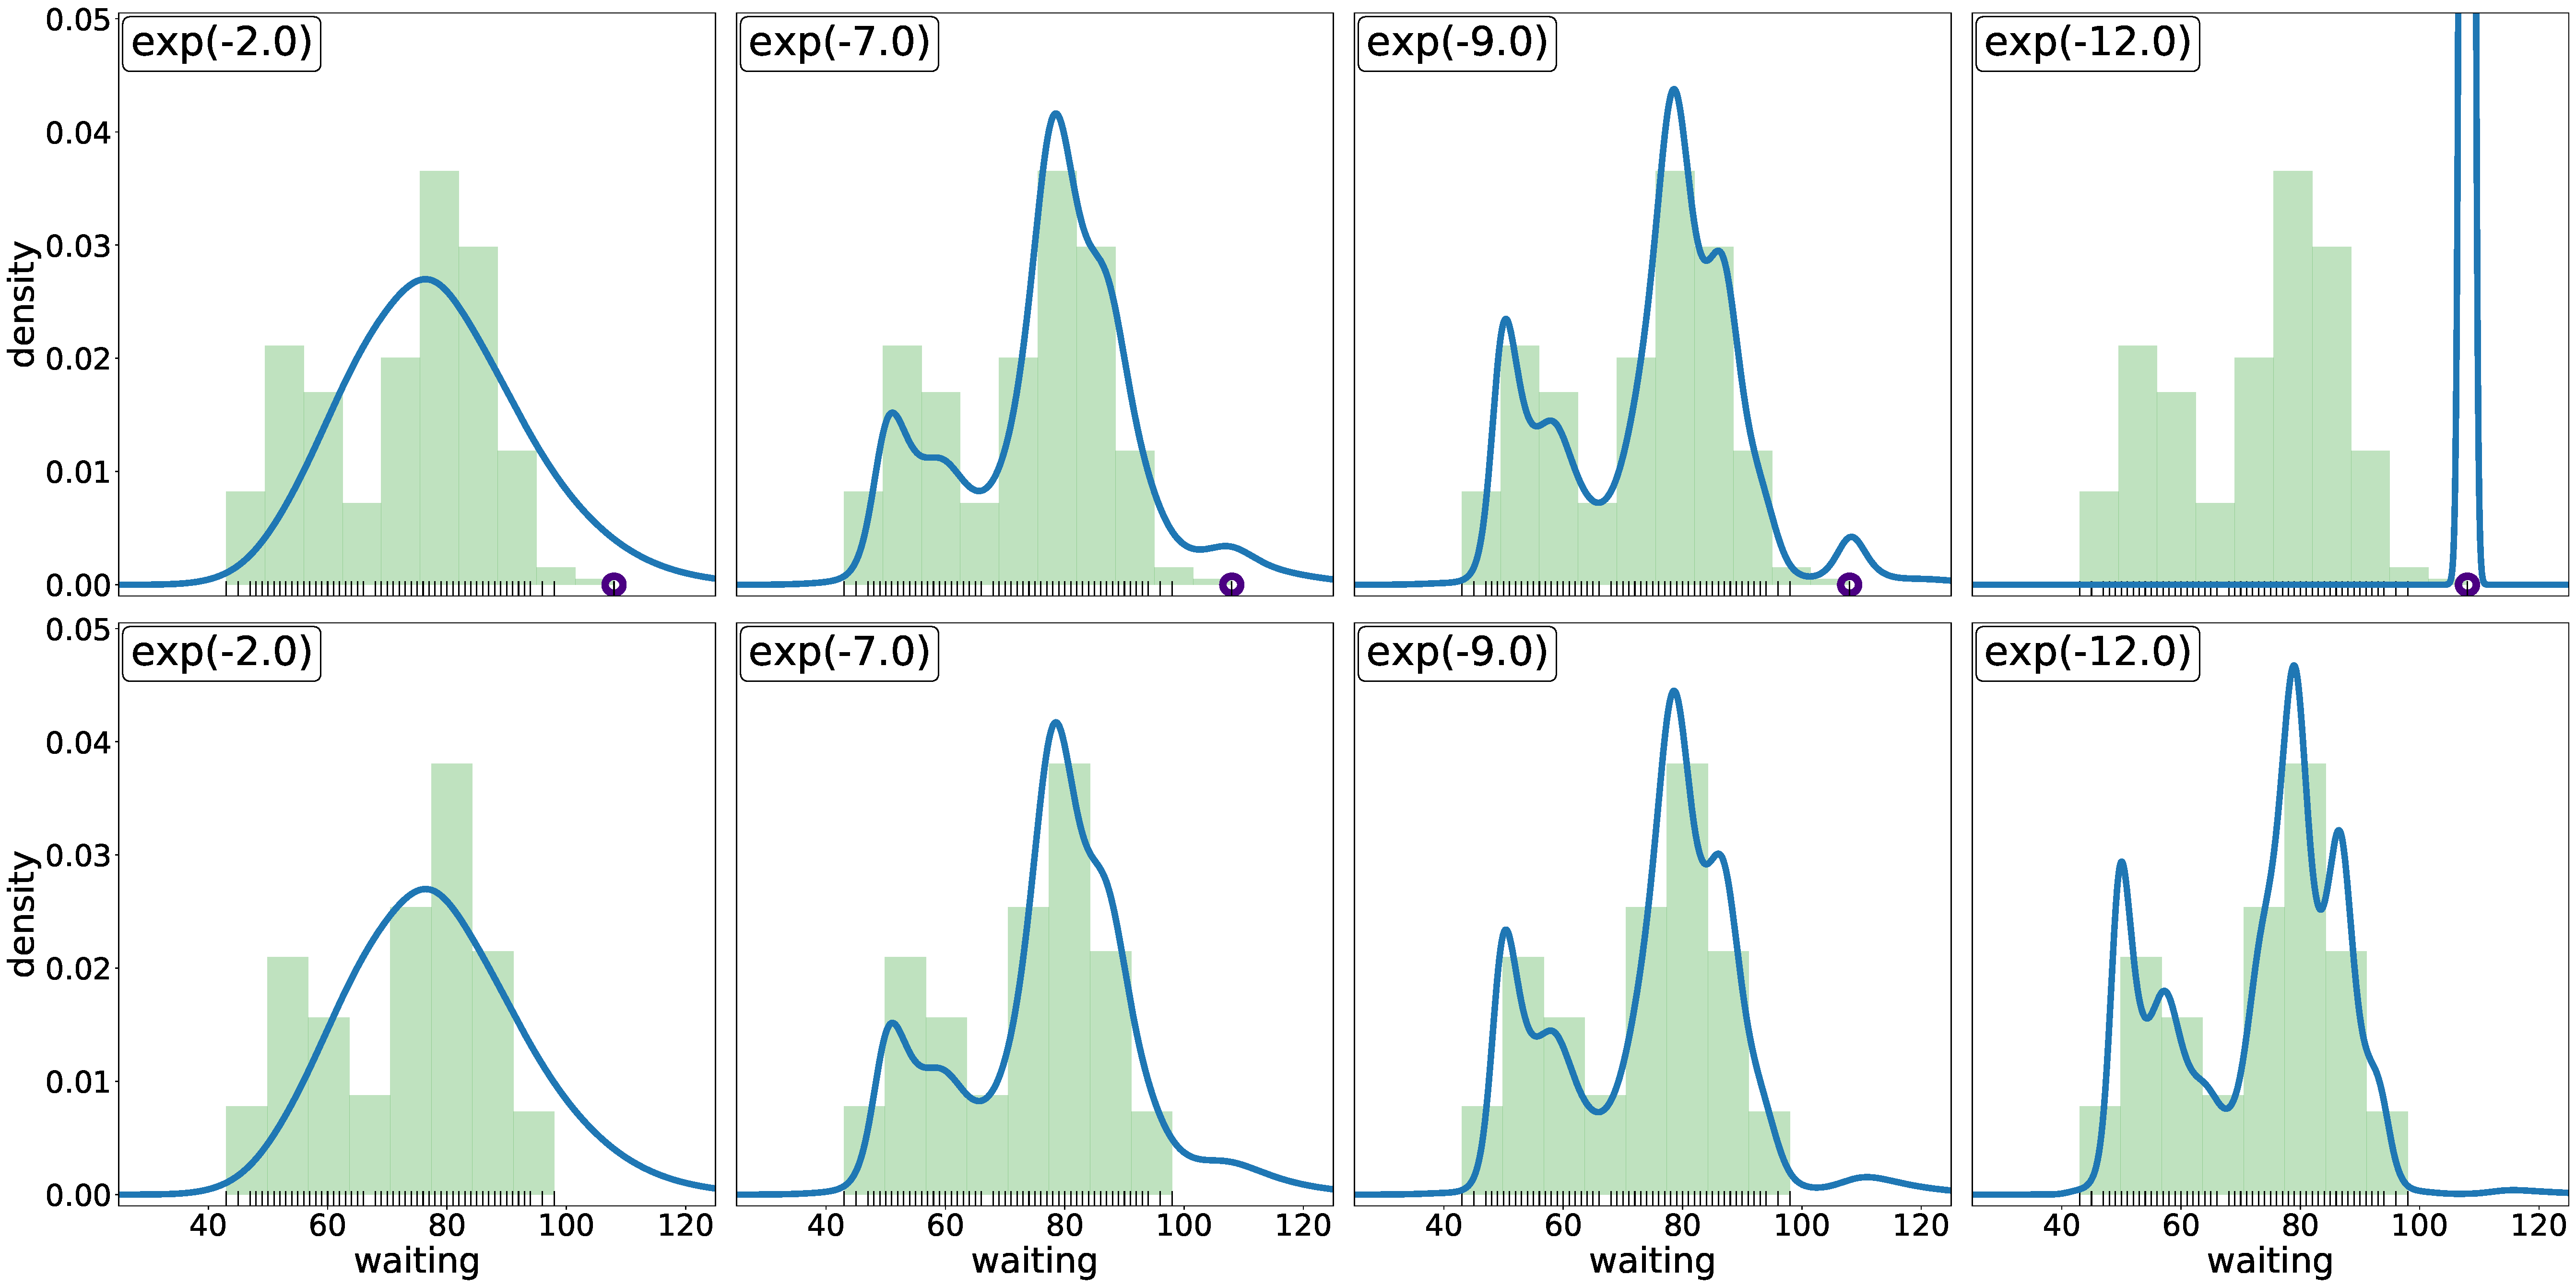
\includegraphics[width=\textwidth]{../plots/waiting-PenSMonly-density-estimates-baseden=Gamma-26-3-gridpoint=1-181-1-with108-brief.pdf}
	{\setstretch{1.0}\caption{Penalized SM density estimates of \texttt{waiting} data with (first row) and without (second row) the isolated observation 108 (indicated by the purple circle). Histogram of the \texttt{waiting} data with the bin width selected by the Freedman-Diaconis rule \textcite{Freedman1981-oi} is shown in green. }
	\label{fig-intro-1}}
\end{figure}

The observations above motivate us to study the sensitivity of these different density estimators to the presence of an isolated observation. The tool we choose is the influence function \parencite{Hampel1968-gm}, a classic concept from the robust statistics. Traditionally, the influence function was defined for real- and vector-valued statistical functionals and was used to study the robustness properties of various real- and vector-valued estimators. But the object of the primary interest in the density estimation problem is a function. The classic notion of the influence is not directly applicable. We extend it to allow function-valued statistical functionals and to facilitate our understanding of the sensitivity of various density estimators. 


\section{Organization of the Remaining Dissertation}\label{section-organization}

The rest of this dissertation is organized as follows. 

In \textbf{\color{red}Chapter 2}, we will formally introduce the kernel exponential family, the family of pdfs in which we estimate $p_0$, discuss its properties, show its connection with the classic finite-dimensional exponential family, and discuss the density estimation problem in it using $\widehat{L}_{\NLL}$ and $\widehat{L}_{\SM}$ found in the literature. 

In \textbf{\color{red}Chapter 3}, we will focus on the early stopping SM density estimator and discuss its theoretical properties. We also compare it with the penalized SM density estimator and address their similarities, both theoretically and empirically. 

In \textbf{\color{red}Chapter 4}, we will compare two kinds of regularized SM density estimators with the penalized ML density estimator. We will provide a specific example to demonstrate that the representer theorem, a classic theorem that characterizes the minimizer of a penalized convex loss functional over a possibly infinite-dimensional RKHS, when applied to minimizing the penalized NLL loss functional fails. Instead, we discuss how to find a finite-dimensional subspace in $\calH$ to approximate the minimizer of the penalize NLL loss functional, and propose an algorithm to compute the minimizer in such a subspace. In addition, we discuss how to compute the regularized SM density estimators in this finite-dimensional subspace. Furthermore, we will explain why the regularized SM density estimators contain a bump or a spike at the isolated observation when there is very small amount of regularization. 

In \textbf{\color{red}Chapter 5}, we will discuss our approach of extending the classic notion of the influence function to the studies of the sensitivity of density estimators. We will study the influence function of ML and SM density projections (to be defined) and estimators in each of finite-dimensional and kernel exponential families. With the comparison of the sensitivity of the ML and SM density estimators, we will also discuss which density estimator should be used and how it should be used in practice. 

Finally, in \textbf{\color{red}Chapter 6}, we will summarize this dissertation and discuss possible future directions based on the current work. 

\newpage

\printbibliography

\end{document}
